\Chapter{Koordináta rendszerek}

Négyzet
Négyzetrács esetében egy derékszögû koordinátarendszer használata a legkézenfekvõbb. 

A derékszögû koordináta-rendszert két egymásra merõleges számegyenes alkotja. Az egyeneseket koordinátatengelyeknek, metszéspontjukat kezdõpontnak, origónak nevezzük. Az origóhoz mindkét számegyenesen a 0-t rendeljük hozzá. A vízszintes tengely az x (abszcissza) tengely, a függõleges az y (ordináta) tengely.

A koordináta-rendszer segítségével a sík bármely P pontjának a helyzete két jelzõszám (koordináta) segítségével egyértelmûen meghatározható. A pont helyzetét a két tengelytõl mért elõjeles távolságával határozzuk meg. A pontnak a tengelyektõl mért elõjeles távolságai a pont koordinátái (jelzõszámai). Az elõjelek a számegyenesek segítségével adhatók meg. A jelzõszámokat, a pont neve után zárójelben adjuk meg: P(x;y).
Hexagon
A hexagonháló esetében többfajta megközelítés is szóbajöhet, most ezek közül fogok néhányat ismertetni. 
Eltolásos koordináta rendszer (Offset coordinates)

	A leggyakoribb megközelítés az eltolásos módszer, ami kisebb eltérésektõl eltekintve gyakorlatilag megegyezik a négyzet koordináta rendszerrel. 

Ha megnézzük a lenti képet, akkor láthatjuk, hogy a hexagonhálóhoz hasonló hatást kapunk, ha a négyzethálóban minden páros/páratlan sort/oszlopot eltolunk.

Eltolható a páros és a páratlan oszlop/sor is. Mivel kétféleképpen is állhatnak a hexagonok, ezért 4 fajta variáció érhetõ el összesen.
		
Kocka koordináta rendszer (Cube coordinates)

	A kocka koordináta rendszerben az eddig megszokottakkal ellentétben nem kettõ, hanem három fõ tengely van.

Tengely koordináta rendszer (Axial coordinates)
IV. Ábrázolás
Négyzet

B. Hexagon

A hexagonok alapvetõen kétféleképpen állhatnak. 
Az egyik lehetõség, hogy az egyik csúcs van felül;
a másik lehetõség, hogy az egyik oldal van felül. 

A következõ lépésként vizsgáljuk meg, hogy hogyan tudjuk egymás mellé elhelyezni a hexagonokat.

A felül hegyes elrendezés esetén vízszintesen a hexagon szélességével, függõlegesen pedig a hexagon magasságának a 3 -vel kell eltolni következõ hexagont. Ezen kívül minden páros/páratlan sort vízszintesen a szélesség felével kell még eltolni.

A felül lapos elrendezés esetén vízszintesen az egymás melletti hexagonok közötti távolság a hexagon szélességének 3 része. Függõlegesen minden páros/páratlan oszlopot a magasság felével kell eltolni.


piros szöveg - kérdéses
kék szöveg - kód

\chapter{A különböző rácsok a játékokban}

\section{Rácsok összehasonlítása}

\begin{figure}[h]
\centering
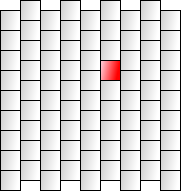
\includegraphics[scale=0.7]{kepek/image13.png}
\caption{}
\label{fig:image13}
\end{figure}

\begin{figure}[h]
\centering
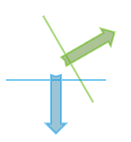
\includegraphics[scale=0.7]{kepek/image14.png}
\caption{}
\label{fig:image14}
\end{figure}

\begin{figure}[h]
\centering
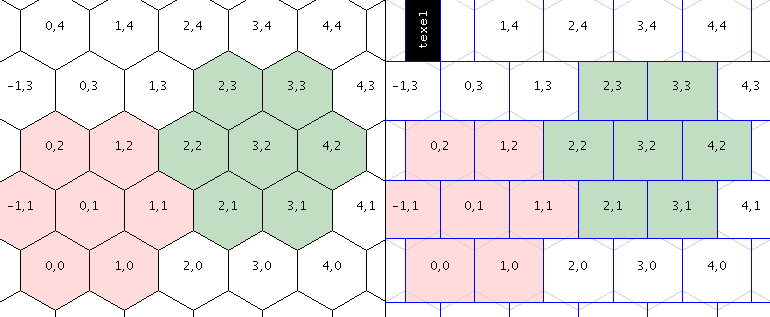
\includegraphics[scale=0.7]{kepek/image15.png}
\caption{}
\label{fig:image15}
\end{figure}

\begin{figure}[h]
\centering
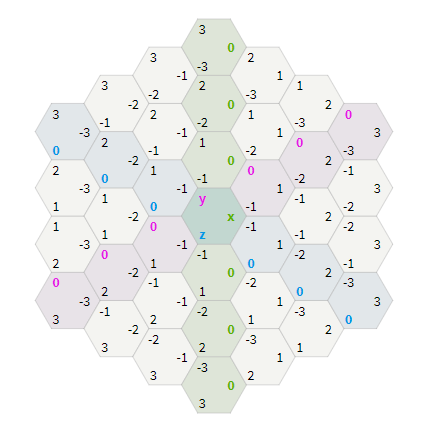
\includegraphics[scale=0.7]{kepek/image16.png}
\caption{}
\label{fig:image16}
\end{figure}

\begin{figure}[h]
\centering
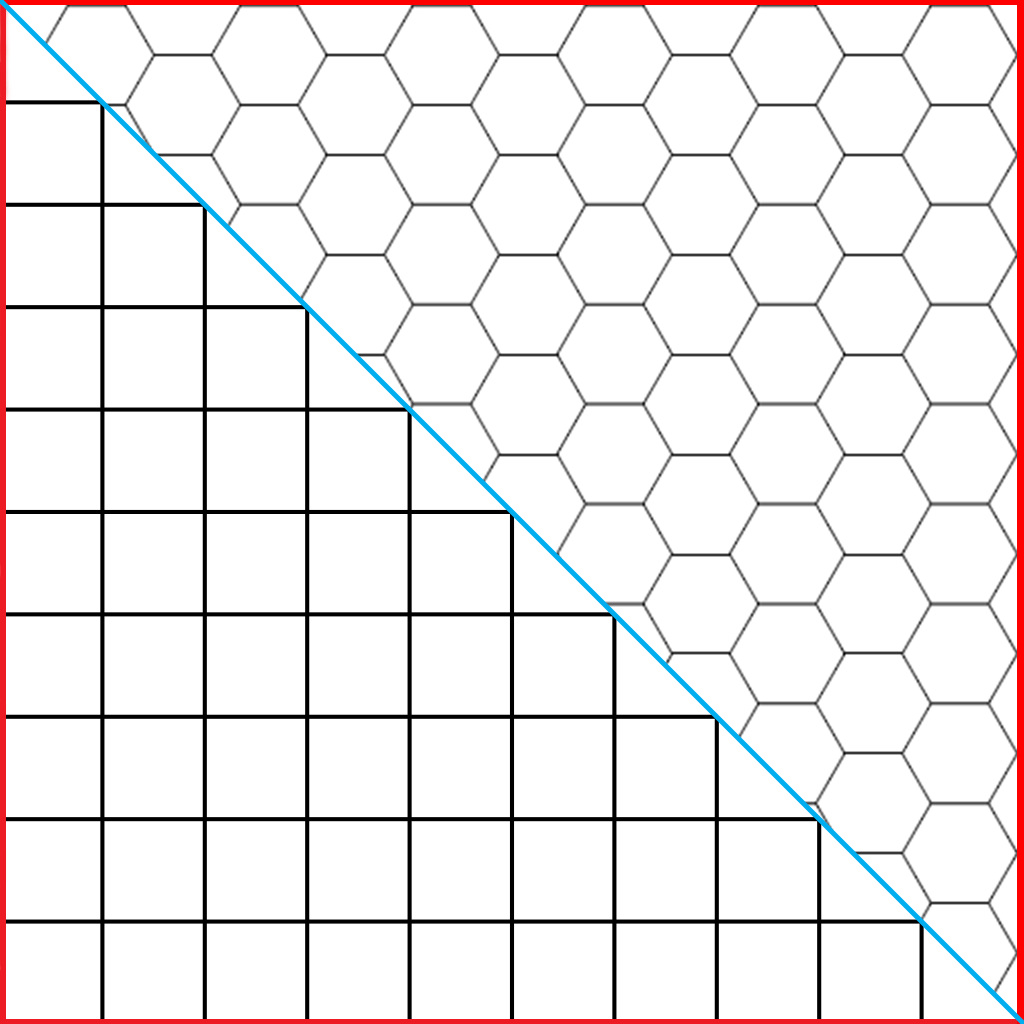
\includegraphics[scale=0.2]{kepek/image22.png}
\caption{}
\label{fig:image22}
\end{figure}

\begin{figure}[h]
\centering
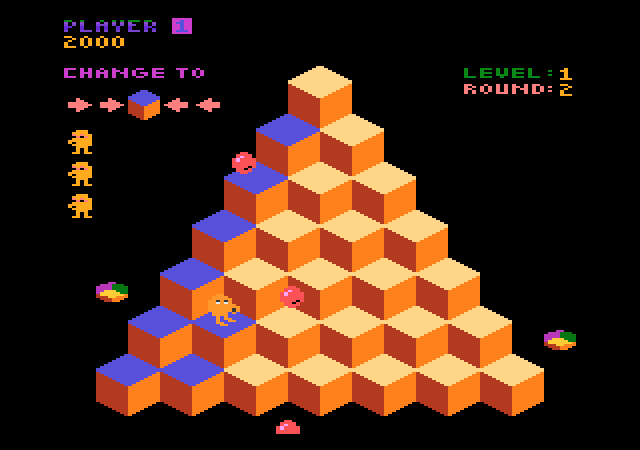
\includegraphics[scale=0.7]{kepek/image23.png}
\caption{}
\label{fig:image23}
\end{figure}

\begin{figure}[h]
\centering
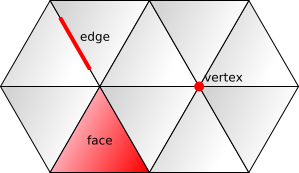
\includegraphics[scale=0.7]{kepek/image24.png}
\caption{}
\label{fig:image24}
\end{figure}

\begin{figure}[h]
\centering
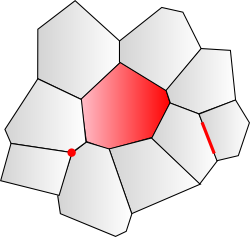
\includegraphics[scale=0.7]{kepek/image25.png}
\caption{}
\label{fig:image25}
\end{figure}

\begin{figure}[h]
\centering
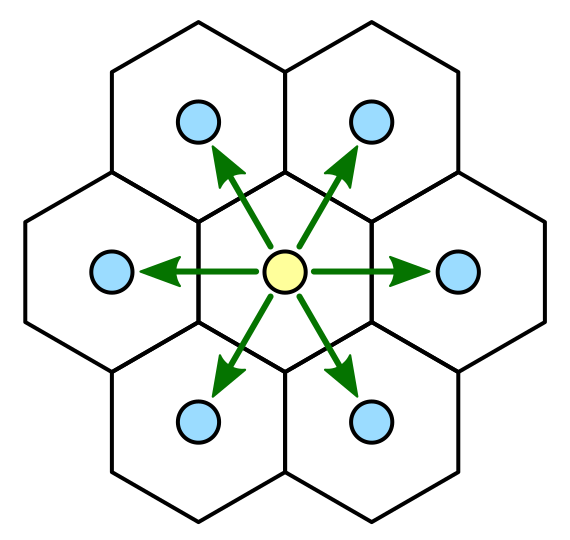
\includegraphics[scale=0.7]{kepek/image26.png}
\caption{}
\label{fig:image26}
\end{figure}

\begin{figure}[h]
\centering
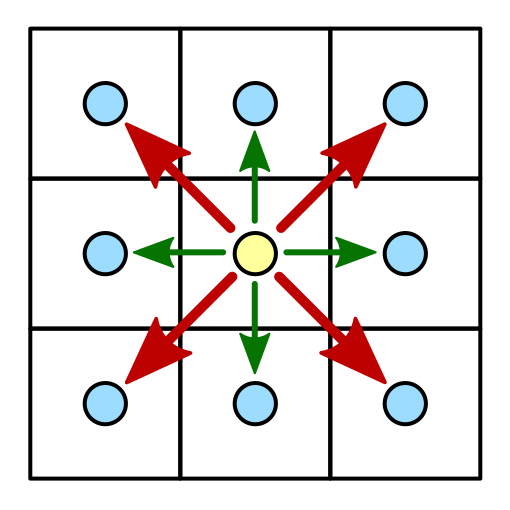
\includegraphics[scale=0.7]{kepek/image27.png}
\caption{}
\label{fig:image27}
\end{figure}

\begin{figure}[h]
\centering
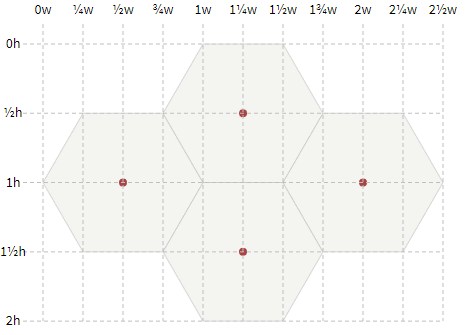
\includegraphics[scale=0.7]{kepek/image28.png}
\caption{}
\label{fig:image28}
\end{figure}

\begin{figure}[h]
\centering
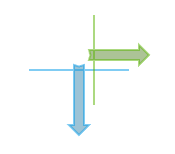
\includegraphics[scale=0.7]{kepek/image4.png}
\caption{}
\label{fig:image4}
\end{figure}

\begin{figure}[h]
\centering
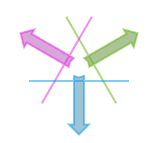
\includegraphics[scale=0.7]{kepek/image5.png}
\caption{}
\label{fig:image5}
\end{figure}

\begin{figure}[h]
\centering
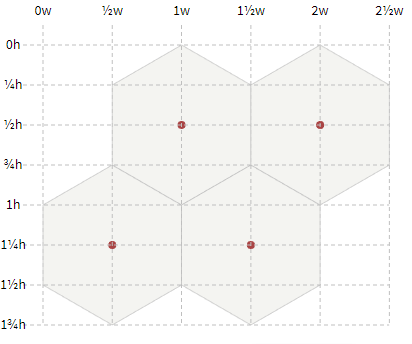
\includegraphics[scale=0.7]{kepek/image8.png}
\caption{}
\label{fig:image8}
\end{figure}

Legyen szó társasjátékról vagy számítógépes játékról, az egyik leggyakrabban használt rács a négyzetrács. Egyszerű, könnyen kezelhető és jól illeszthető a számítógép kijelzőjére. A cellák pozícióit a Descartes-féle derékszögű koordináta-rendszer $(x, y)$ segítségével határozhatjuk meg. Kirajzolásához ismernünk kell a cellai méreteit (szélesség, magasság) illetve a rács méreteit (oszlopok, sorok száma). A nyilvántartáshoz ismernünk kell a viszonyítási pontot (origó), illetve tudnunk kell az objektum pozicióját $(x, y)$.

Könnyen kezelhetősége mellett viszont van egy nagy hátránya:
Egy négyzetnek nyolc szomszédja van. Oldalain keresztül vízszintesen, valamint függőlegesen 2-2 szomszédja érhető el. További négy szomszédja átlósan található meg. A problémára akkor figyelünk fel, amikor megvizsgáljuk a távolságot a különböző szomszédok között. A vizsgálathoz tegyük fel, hogy az oldalak hossza 1. Ha a négyzetek középpontjához viszonyítunk, akkor a függőlegesen és a vízszintesen lévő szomszédok távolsága 1, míg az átlósan lévők távolsága $\sqrt{2}$.

A két fajta szomszéd közötti különbség miatt vetődnek fel bizonyos kérdések:
\begin{itemize}
\item Hogyan kezeljük az átlós mozgást? 
\item Egyáltalán engedélyezzük-e az átlós mozgást? 
\end{itemize}

A problémára több megoldás is létezik:

Nem alkalmazunk átlós mozgást. Ez a legegyszerűbb megoldás, amit az egyszerűsége miatt gyakranhasználnak

Egy kevésbé elterjedt megoldás, hogy maradunk a négyzeteknél, viszont minden második sort/oszlopot eltolunk az oldal szélességének/hosszának a felével. Ekkor az összes szomszéd hasonló távolságra kerül.

3. A leggyakoribb megoldás a hexagonok használata a négyzetek helyett. A négyzethez hasonlítva a hatszögnek csak hat szomszédja van (nyolc helyett). Ezek közül mindegyik oldal szomszéd, és nincs olyan szomszédja ami a sarkokhoz esne. Ezáltal minden szomszéd egyenlően 1 távolságra van.

A hexagonokat azért szokták játékokban használni mert kevésbé torzítják a távolságokat mint a négyzetrács. Ez azért van mert nincs átlós szomszédja ellentétben a négyzettel. (Az átlós szomszédok torzítják a távolságokat.)

A fő indok a hexagonháló mellett az eltolt négyzethálóval szemben az, hogy sokkal kézenfekvőbb a hat lehetséges mozgási iránynak a használata. Emelett még eszétikailag is kellemesebb érzeted nyújt a felhasználó számára.

\section{Rácsok felhasználása}

Alapvetően mindkét rácsnak megvan a maga helye a játékokban. 

Mivel a beltéri helyszínek (szobák) és az azon belüli elemek (bútor) általában téglalap alakúak, praktikusabb a négyzetrács használata. A négyzetrács a falakhoz tökéletesen illeszkedik, ugyanakkor a hexagonok esetében problémák merülnek fel. Ugyanis a hexagonok nem fognak szabályosan illeszkedni a falak mentén. Erre kétfajta megoldás létezik: a fal menti hexagonokat elvághatjuk, vagy másik megoldás, ha nem töltjük ki a fennmaradó helyeket. Egyik megoldással sem lehetünk maradéktalanul elégedettek, ha elvágjuk a hexagonokat. 

Akkor azok hogyan viselkedjenek? 
Lehessen-e rálépni?
Ha nem lehet rálépni akkor miért van?

Ha csak kihagyjuk a széleken a hexagonokat amik nem férnek el az a felhasználó számára furcsa összhatást nyújthat.

Ha mindenképpen hexagonokat  szeretnénk használni kis méretű térképen (pl: $8 \times 20$), akkor lehetőleg ne egy zárt szobában alkalmazzuk hanem szabad téren (pl: mező, erdő, tenger part) vagy próbáljuk a hexagon rács széleihez igazítani a környezetet.

Kültéren, falak hiányában ezek a problémák nem merülnek fel. Emiatt, valamint a négyzetrács átlós mozgásával kapcsolatos problémák miatt előnyösebb a hexagonháló használata ezekben az esetekben.

\section{Rácsok Részei}

A rácsoknak három különböző része van: a lap (face), élek és csúcsok. Minden lap két dimenziós felület élek által határolva. Minden él egy dimenziós szakasz aminek mind a két végén csúcsok találhatóak. Minden csúcs nulla dimenziós pont. 

A játékok nagy többségében közös az, hogy a rácsoknak csak az egyik részére koncentrálnak. A nyugati játékoknál mint a sakk vagy a dáma a rácsnak a lap részén van a fókusz ellentétben a keleti játékokkal mint a go vagy a csillaghalma (Chinese Checkers) 

Lapok, élek és a csúcsok feltűnnek a különböző poligonokból álló  térképek esetén is. Az algoritmus ami a lapok, élek vagy csúcsok alapján működik de nincs szükség koordinátákra az működni fog poligoniális térképek esetén is.

A rácsok és a poligoniális térképek átalakíthatóak gráf struktúrákra azáltal, hogy minden lapból csomópontot és minden lapok közötti élből pedig a csomópontok közötti gráf éleket készítünk. A gráf struktúra, hogy gráf algoritmusokat (például: legrövidebb út) használjunk a térképen.
Használatuk játékokban
A számítógépes játékok mind a három tipust használhatják, de a lap a leggyakoribb. Épületek, terület tipusok (fű, sivatag, stb.) és a terület birtoklás a lapokat használja. Terület határok és az “áramlás” (“flow”) algoritmusok (ami szimulálja az áramlását a víznek, embereknek, termékeknek, stb. a szomszédos csempék között) használják az éleket. Az utakhoz lehet használni a lapokat és az éleket is.

\section{Koordináta rendszerek}

Négyzet
Négyzetrács esetében egy derékszögű koordinátarendszer használata a legkézenfekvőbb. 

A derékszögű koordináta-rendszert két egymásra merőleges számegyenes alkotja. Az egyeneseket koordinátatengelyeknek, metszéspontjukat kezdőpontnak, origónak nevezzük. Az origóhoz mindkét számegyenesen a 0-t rendeljük hozzá. A ,,vízszintes'' tengely az $x$ (abszcissza) tengely, a ,,függőleges'' az $y$ (ordináta) tengely.

A koordináta-rendszer segítségével a sík bármely P pontjának a helyzete két jelzőszám (koordináta) segítségével egyértelműen meghatározható. A pont helyzetét a két tengelytől mért előjeles távolságával határozzuk meg. A pontnak a tengelyektől mért előjeles távolságai a pont koordinátái (jelzőszámai). Az előjelek a számegyenesek segítségével adhatók meg. A jelzőszámokat, a pont neve után zárójelben adjuk meg: $P(x;y)$.

Hexagon

A hexagonok hat oldalú poligonok. A szabályos hatszögnek minden oldala egyenlő hosszúságú. A szakdolgozatomban csak szabályos hatszögekkel fogok foglalkozni. 

Egy hexagonnak hat oldala van. Minden oldalon két hexagon osztozik. A hexagonoknak hat csúcsa van, Minden csúcson 3 hexagon osztozik.

A hexagonháló esetében többfajta megközelítés is szóbajöhet, most ezek közül fogok néhányat ismertetni. 
Eltolásos koordináta rendszer (Offset coordinates)

	A leggyakoribb megközelítés az eltolásos módszer, ami kisebb eltérésektől eltekintve gyakorlatilag megegyezik a négyzet koordináta rendszerrel. 

A négyzethálóval is elérhetünk a hexagonhálóhoz hasonló hatást, ha a négyzethálóban minden páros/páratlan sort/oszlopot eltolunk.

Eltolható a páros és a páratlan oszlop/sor is. Mivel kétféleképpen is állhatnak a hexagonok, ezért 4 fajta variáció érhető el összesen.

A négyzet koordinátarendszerhez hasonlóan itt is a hálónk egyik sarka lesz a kezdő pont (origó) amihez viszonyítva számozzuk majd a sorokat és oszlopokat.

Az eltolásos kooridinátarendszernek az egyik hátránya, hogy a kettőből az egyik tengelye mentén nem egyenesen halad a hexagonok az eltolás miatt, ezáltal bonyolítva a dolgokat. A további rendszerek ezt a problémát orvosolják, viszont ott más problémák merülnek fel.		
Kocka koordináta rendszer (Cube coordinates)

Egy másik fajta megközelítésből nézzük a hexagon hálókat, akkor láthatjuk, hogy három elsődleges tengelye van, nem úgy mint a korábbi koordinátarendszereknek. 

Ahhoz, hogy megértsük a kocka koordináta rendszert képzeljünk el egy kockarácsot és vágjunk ki belőle egy átlós síkot az x + y + z = 0 mentén. Ez fogja majd a hexagon rácson használt algoritmusokat egyszerűbbé tenni. Azáltal, hogy használhatjuk a Descartes-féle koordináta-rendszerben való műveleteket: hozzáadás a koordinátákhoz, kivonás a koordinátákból, szorzás vagy osztás skalárral, távolság számítás.

Egy szemléletesebb példaként vizsgáljuk meg a Q*bert nevű játékot.

A játék egy 28 kockából álló piramis szerű játékmezőn zajlik (Ilyen alakzatot kapunk, ha végrehajtjuk a fent írtakat.). A játékos Q*bert-et (narancssárga karakter) irányítja, aki, ha ráugrik egy kockára akkor átszinezi azt.

Ha jobban megfigyeljük az ábrát, akkor láthatjuk, hogy a kockák valójában hexagonok, ha 2D-ben rendereljük, ha így nézzük, akkor Q*bert 6 különböző irányba is léphet. Ez azt jelenti, hogy a párhuzamosan lévő oldalakra merőlegesen helyezünk tengelyeket, akkor hármat tudunk elhelyezni 120 fokonként.

Minden hexagonnak 3 koordinátája van. 
Mindegyik tengely egy egyenes vonalnak felel meg a hexagon hálón.
Minden irány a hexagonon másik két iránynak a kombinációja a kocka koordináta rendszeren. Például, ha a (*ábra megnevezése) ábrán felfelé szeretnénk mozogni, akkor az a +y és -z között fekszik, ezért minden lépésnél ami felfelé történik hozzá kell adnunk 1-et az y-hoz és el kell vennünk 1-et a z-ből. 

Ez azért történik mert minden egyes mező koordinátájának az összege 0 kell, hogy legyen (x + y + z = 0). Ez azt is jelenti, hogy a harmadik tengely bizonyos esetekben redundáns is lehet, például amikor meghatározzuk, hogy az egyes mezők hol jelenjenek meg a képernyőn, ugyanakkor olyan esetekben mint az útkereső vagy a távolság számító algoritmusok az előnye egyértelműen látszik. 

Tengely koordináta rendszer (Axial coordinates)

Tengely koordinátarendszer csak kettő koordinátát használ a kocka koordinátarendszer három koordinátája közül. Mivel a kocka koordinátarendszernél volt az a megkötés, hogy x + y + z = 0, és ahogy már a kocka koordinátarendszernél már leírtam a harmadik koordináta redundáns.  A tengelyes koordinátarendszer használható tárolásra és megjelenítésére és mivel az x + y + z = 0 egyenlet alapján kiszámítható a harmadik koordináta ezért a számításokhoz is könnyen használható.

Az előnye ennek a rendszernek az eltolásoshoz képest, hogy az algoritmusok egyszerűbbek. A hátránya ennek a rendszernek a téglalap alakú térképek esetén való tárolás. 
V. Koordináta konverziók
Mivel a tárolás, megjelenítés és a számítások nem ugyanabban a koordináta rendszerben fog megvalósulni, ezért szükséges ismernünk a különböző konverziós eljárásokat oda-vissza a különböző rendszerek között. Mivel a számításokhoz a kocka koordinátarendszert fogom alkalmazni, ezért erre a rendszerre fogom alapozni az algoritmusokat.

Tengelyes - Kocka konverziók
A tengelyes koordináta rendszer nagyon közel áll a kocka koordináta rendszerhez. A tengelyes csak elhagyja a harmadik koordinátát, a kocka pedig kiszámolja a harmadikat a másik kettő alapján.

\begin{verbatim}
function cube_to_axial(cube):
    var q = cube.x
    var r = cube.z
    return Hex(q, r)

function axial_to_cube(hex):
    var x = hex.q
    var z = hex.r
    var y = -x-z
    return Cube(x, y, z)
\end{verbatim}

2. Eltolásos - Kocka konverziók
Az eltolásos koordináta rendszernek négy fajta tipusa lehet, az alapján, hogy melyik sor/oszlop lett eltolva.

Páratlan - sor:

\begin{verbatim}
function cube_to_oddr(cube):
      col = cube.x + (cube.z - (cube.z&1)) / 2
      row = cube.z
      return Hex(col, row)

function oddr_to_cube(hex):
      x = hex.col - (hex.row - (hex.row&1)) / 2
      z = hex.row
      y = -x-z
      return Cube(x, y, z)
\end{verbatim}

Páros - sor:

\begin{verbatim}
function cube_to_evenr(cube):
      col = cube.x + (cube.z + (cube.z&1)) / 2
      row = cube.z
      return Hex(col, row)

function evenr_to_cube(hex):
      x = hex.col - (hex.row + (hex.row&1)) / 2
      z = hex.row
      y = -x-z
      return Cube(x, y, z)
\end{verbatim}      
      
Páratlan - oszlop:

\begin{verbatim}
function cube_to_oddq(cube):
      col = cube.x
      row = cube.z + (cube.x - (cube.x&1)) / 2
      return Hex(col, row)
\end{verbatim}

\begin{verbatim}
function oddq_to_cube(hex):
      x = hex.col
      z = hex.row - (hex.col - (hex.col&1)) / 2
      y = -x-z
      return Cube(x, y, z)
\end{verbatim}

Páros - oszlop:

\begin{verbatim}
function cube_to_evenq(cube):
      col = cube.x
      row = cube.z + (cube.x + (cube.x&1)) / 2
      return Hex(col, row)
\end{verbatim}

\begin{verbatim}
function evenq_to_cube(hex):
      x = hex.col
      z = hex.row - (hex.col + (hex.col&1)) / 2
      y = -x-z
      return Cube(x, y, z)
\end{verbatim}


\section{Ábrázolás}

Négyzet
A négyzetháló esetén van a legkönnyebb dolgunk ismént. A négyzetek alapvetően egy féle képpen állnak, úgy, hogy a lapjunk áll felfelé.  A négyzeteket ebben az esetben, úgy tudjuk egymás mellé helyezni, hogy a szomszédos négyzetek középpontjai közötti távolság megegyezik az oldal hosszal. 

Abban az esetben sincs sokkal nehezebb dolgunk, ha úgy döntünk, hogy az eltolt négyzetrácsos megoldást választjuk, ebben az esetben minden páros/páratlan sort/oszlopot kell eltolnunk az oldalhosszának felével.
B. Hexagon

A hexagonok alapvetően kétféleképpen állhatnak. Az egyik lehetőség, hogy az egyik csúcs van felül, a másik lehetőség, hogy az egyik oldal van felül. 

A következő lépésként vizsgáljuk meg, hogy hogyan tudjuk egymás mellé elhelyezni a hexagonokat.

A felül hegyes elrendezés esetén vízszintesen a hexagon szélességével, függőlegesen pedig a hexagon magasságának a $\dfrac{3}{4}$ részével kell eltolni következő hexagont. Ezen kívül minden páros/páratlan sort vízszintesen a szélesség felével kell még eltolni.

A felül lapos elrendezés esetén vízszintesen az egymás melletti hexagonok közötti távolság a hexagon szélességének $\dfrac{3}{4}$ része. Függőlegesen minden páros/páratlan oszlopot a magasság felével kell eltolni.

\section{Távolság számítás}

1. Kocka koordinátarendszer
A kocka koordináta rendszerben, minden hexagon egy kockának felel meg a 3D térben. A szomszédos hexagonok 1 távolságra vannak egymástól a hexagonháló esetén, viszont 2 távolságra vannak egymástól a kocka koordinátarendszerben. Ezáltal téve egyszerűvé a távolságszámítást. A négyzet koordinátarendszer esetén a Manhattan távolság képlet a következő: abs(dx) + abs(dy). A kocka koordinátarendszerben pedig a Manhattan távolság abs(dx) + abs(dy) + abs(dz). Ezekből következik, hogy a hexagon rács esetén a Manhattan távolság képlet a kockarács esetén fentálló távolság fele.

Pseudo kóddal:

\begin{verbatim}
function cube_distance(a, b):
    return (abs(a.x - b.x) + abs(a.y - b.y) + abs(a.z - b.z)) / 2
\end{verbatim}

$$
d_{\text{cube}}(a, b) =
\dfrac{|a_x - b_x| + |a_y - b_y| + |a_z - b_z|}{2}
$$

Egy ezzel egyenértékű megközelítés az is, ha megfigyeljük azt, hogy a három koordináta közül az egyiknek mindenképpen a a másik kettő összegének kell, hogy legyen, ekkor az az egy lesz a távolság. 

Pseudo kóddal:
\begin{verbatim}
function cube_distance(a, b):
    return max(abs(a.x - b.x), abs(a.y - b.y), abs(a.z - b.z))
\end{verbatim}

$$
d_{\text{cube}}(a, b) =
\max(
|a_x - b_x|, |a_y - b_y|, |a_z - b_z|
)
$$

Az, hogy melyik algoritmust váltjuk az szituáció és egyén függő, de az eredmény ugyanaz.
Tengelyes koordinátarendszer
Eltolásos koordinátarendszer

\section{Útkereső algoritmus}

A hexagonok és a négyzetek esetén az útkeresés csak egy ponton különbözik (szomszédok száma) ezért az egyszerűség kedvért csak a négyzethálónál mutatom be.

Az algoritmus: 

\begin{verbatim}
OPEN //the set of nodes to be evaluated
CLOSED //the set of nodes already evaluated
add the start node to OPEN

loop
	current = node in OPEN  with the lowest f_cost
remove current from OPEN
add current to CLOSED

if current is the target node //path has been found
return

foreach neighbour of the current node
	if neighbour is not traversable or neighbour is in CLOSED
skip to the next neighbour

if new path to neighbour is shorter OR neighbour is not in OPEN
set f_cost of neighbour
set parent of neighbour to current
if neighbour is not in OPEN
add neighbour to OPEN
\end{verbatim}

Szomszédok

Ahhoz, hogy útkereső algoritmust tudjunk készíteni ismernünk kell, hogy a különböző alakzatok és koordináta rendszerek esetén milyen algoritmussal érhetjük el az adott alakzat szomszédait. 

Az algoritmusokat ebben a formában fogom megadni: A -> B1, B2, B3 …
(Az “A” és “B” pontokat “u”, “v” koordináták segítségével fogom megadni.)
Négyzet
A négyzet esetén egyszerű dolgunk van, mert csak egyfajta koordináta rendszerünk van.

$$
(u,v) \Rightarrow (u,v+1) (u+1,v) (u,v-1), (u-1,v)
$$

Hexagon

Hexagon esetén több fajta koordináta rendszerünk is lehet.
Kocka koordináta rendszer (Cube coordinates)
Ahhoz, hogy elmozduljunk eggyel meg kell változtatnunk egyet a három kocka koordináta közül +1-el és egy másikat -1-el (a változtatások összege 0 kell, hogy legyen). Három koordinátát lehet megváltoztatni +1-el, a másik két lehetséges koordináta közül az egyiket kell csökkenteni -1-el. Ez hat lehetséges változatot eredményez. Mindegyik megfeleltethető a hexagon egyik irányának. A lehető legegyszerűbb és leggyorsabb megoldás az, ha az összes lehetséges permutációt előre kikalkuláljuk és beleírjuk egy táblázatba ( Cube(dx, dy, dz)).

\begin{verbatim}
var cube_directions = [
   Cube(+1, -1,  0), Cube(+1,  0, -1), Cube( 0, +1, -1),
   Cube(-1, +1,  0), Cube(-1,  0, +1), Cube( 0, -1, +1)
]

function cube_direction(direction):
    return cube_directions[direction]

function cube_neighbor(cube, direction):
    return cube_add(cube, cube_direction(direction))
\end{verbatim}

Tengely koordináta rendszer (Axial coordinates)
A kocka koordináta rendszer veszük alapul. Mégpedig úgy, hogy a Cube( dx, dy, dz) koordinátákat átalakitjuk Axial( dx, dz) -re.

\begin{verbatim}
var axial_directions = [
   Hex(+1,  0), Hex(+1, -1), Hex( 0, -1),
   Hex(-1,  0), Hex(-1, +1), Hex( 0, +1)
]

function hex_direction(direction):
    return axial_directions[direction]

function hex_neighbor(hex, direction):
    var dir = hex_direction(direction)
    return Hex(hex.q + dir.q, hex.r + dir.r)
\end{verbatim}

Eltolásos koordináta rendszer (Offset coordinates)
Eltolásos koordináta rendszer esetén a lépések változnak annak a függvényében, hogy hol állunk a hálóban. Ha mi egy eltolt oszlopban/sorban állunk akkor a szabály eltér attól mintha egy nem eltolt oszlopban/sorban állnánk.

Ahogy a korábbi esetekben úgy most is kell készítenünk egy táblázatot amiben azt tároljuk majd, hogy a különböző tengelyeken mennyit kell hozzáadni, hogy elérjük a szomszédokat. De ebben az esetben most két tömbre lesz szükségünk, az egyik a páros sor/oszlop a másik pedig a páratlan sor/oszlop esetére.

A táblázat különbözik mind a négy eltolásos módszernél.

Páratlan sor

\begin{verbatim}
var oddr_directions = [
   [ Hex(+1,  0), Hex( 0, -1), Hex(-1, -1),
     Hex(-1,  0), Hex(-1, +1), Hex( 0, +1) ],
   [ Hex(+1,  0), Hex(+1, -1), Hex( 0, -1),
     Hex(-1,  0), Hex( 0, +1), Hex(+1, +1) ]
]

function oddr_offset_neighbor(hex, direction):
    var parity = hex.row & 1
    var dir = oddr_directions[parity][direction]
    return Hex(hex.col + dir.col, hex.row + dir.row)
\end{verbatim}

Páros sor

\begin{verbatim}
var evenr_directions = [
   [ Hex(+1,  0), Hex(+1, -1), Hex( 0, -1),
     Hex(-1,  0), Hex( 0, +1), Hex(+1, +1) ],
   [ Hex(+1,  0), Hex( 0, -1), Hex(-1, -1),
     Hex(-1,  0), Hex(-1, +1), Hex( 0, +1) ]
]

function evenr_offset_neighbor(hex, direction):
    var parity = hex.row & 1
    var dir = evenr_directions[parity][direction]
    return Hex(hex.col + dir.col, hex.row + dir.row)
\end{verbatim}

Páratlan oszlop

\begin{verbatim}
var oddq_directions = [
   [ Hex(+1,  0), Hex(+1, -1), Hex( 0, -1),
     Hex(-1, -1), Hex(-1,  0), Hex( 0, +1) ],
   [ Hex(+1, +1), Hex(+1,  0), Hex( 0, -1),
     Hex(-1,  0), Hex(-1, +1), Hex( 0, +1) ]
]

function oddq_offset_neighbor(hex, direction):
    var parity = hex.col & 1
    var dir = oddq_directions[parity][direction]
    return Hex(hex.col + dir.col, hex.row + dir.row)
\end{verbatim}

Páros oszlop

\begin{verbatim}
var evenq_directions = [
   [ Hex(+1, +1), Hex(+1,  0), Hex( 0, -1),
     Hex(-1,  0), Hex(-1, +1), Hex( 0, +1) ],
   [ Hex(+1,  0), Hex(+1, -1), Hex( 0, -1),
     Hex(-1, -1), Hex(-1,  0), Hex( 0, +1) ]
]

function evenq_offset_neighbor(hex, direction):
    var parity = hex.col & 1
    var dir = evenq_directions[parity][direction]
    return Hex(hex.col + dir.col, hex.row + dir.row)
\end{verbatim}

Átlós

\section{Mit választottam és miért}

hexagon
coordinate systems
offset
cube
pointy top
rácsok részei
szomszédok

eltolásos koordináta rendszert fogok használni a megjelnítésben és a tárolásban, mivel ezekre a célokra ez a módszer a legegyszerűbb. A különböző számításokhoz pedig kocka koordináta rendszert fogom alkalmazni.

\section{Megvalósítás}

Modellek létrehozásának módja

Bemenetként a térkép fő jellemzőit, a generált térképpel szembeni elvárásokat kapja paraméterezésként.

A térkép egy több lépcsős folyamat végén fog elkészülni. 
Az első fázisban a nagyobb területi egységek (szigetek, folyók, ...) körvonalazódása történik. 

A második lépésben a térkép alapegységeinek (tile) a konkretizálása történik meg, azaz leképződik egy hexagon háló. 
Harmadik lépésként minden egyes tile-hoz hozzárendeli az algoritmus a megfelelő textúrát a területi egységek alapján. 
A negyedik fázisban városokat, településeket, falakat hoz létre a program. 

Ötödik lépésként a növényzetet (fák, bokrok) generálja majd le. 
A hatodik lépésben a dekorálás jön, ahol az évszakoknak és a különböző természeti hatásoknak megfelelően módosulhat a textúra.

Első lépésként szükségünk lesz egy csempére (tile), ami az alapelem lesz a térképen. Erre a célra én egy 3D-s hexagon modellt használtam különböző textúrákkal.
Ezen kívül szükség van a generálni kívánt térkép méreteire (szélesség, magasság).
